\documentclass[11pt, oneside]{report}
\usepackage[margin=1.5in]{geometry}
\usepackage{setspace}
\usepackage[utf8]{inputenc}
\usepackage{amsmath}
\usepackage{float}
\usepackage{graphicx}
\usepackage{tocbibind}
\usepackage{url}
\usepackage{cite}

\title{Communicating Replicated State Machines}
\author{David Wetterau}
\date{April 2015}

\begin{document}

\maketitle

\tableofcontents

\chapter{Introduction}\label{Introduction}
Computing systems today are rarely self-contained units. 
The desire for more levels of abstraction and cleaner separations of responsibilities has led to systems being modularized into services that must communicate and work together to accomplish tasks. 
Not only is this separation observed within single systems, but also in systems that interact with external services such as cloud based storage or computing providers \cite{tao, spanner, dynamo}. 
In this paper we will present a way to build these systems in a highly available and fault tolerant manner by building upon the existing techniques of State Machine Replication (SMR) \cite{practicalBFT, hq, zyz, paxos, paxosMadeSimple, schneider} and pipelining.

Unfortunately, SMR as it exists today is not immediately fit for an environment where services communicate. 
Previous work on SMR has focused on the client-server model, where a replicated state machine behaves as a single-correct-server from the perspective of the clients making requests \cite{schneider}.
This abstraction explicitly does not consider what separate services communicating with a SMR system observe. This means that separate services could be exposed to inconsistent states across correct replicas which violates the safety property of SMR.

% TODO: make the previous sentence more clear, this is critical to the motivation of this work and Alvisi was confused by it

Aside from consistency issues in an environment with communicating replicated services, traditional SMR also suffers from fundamental performance deficiencies in today's computing environment. 
Many SMR protocols rely on the sequential execution of commands to guarantee that replicas operate in a deterministic manner \cite{practicalBFT, upRight, hq, paxos}. 
Not only does sequential execution do a poor job of leveraging abundantly available multicore machines, it also requires that a system that communicates with other services remain idle while waiting for the response of a request issued to another service.

In this paper, we present a technique to efficiently perform SMR in a system where replicated services must communicate while processing client requests.
We first leverage speculative execution \cite{eve, zyz} to allow our system to be multi-threaded and therefore better utilize the multicore nature of machines today. 
We then show how to pipeline a speculative execution system to avoid unnecessary blocking when waiting for the responses of requests sent to other services.
This work builds on contributions originally made by the Laboratory for Advanced Systems Research at the University of Texas at Austin \cite{eve, manosThesis} and was a joint effort between David Wetterau and Jim Given. 
We highly recommend reading both this thesis and Given's thesis \cite{jim} on this work to get the complete understanding of this project.

The rest of this paper is structured as follows. 
Chapter \ref{Background} provides a comprehensive background on the replicated state machine abstraction and the Eve system, which pioneered the use of multi-threaded speculative execution in an SMR system. 
Chapter \ref{Adam} introduces Adam, a system to provide high availability in an environment with services that communicate not only with clients, but also with other services. 
Chapter \ref{AdamDesign} describes at a high level the design and benefits of multi-threaded pipelining in Adam. 
Chapter \ref{AdamImplementation} explains our implementation of Adam in detail along with the correctness guarantees Adam provides. 
Chapter \ref{AdamResults} displays our evaluation and the performance of Adam. 
Chapter \ref{FutureWork} explains some of the future directions we believe would be fruitful for this system.
Chapter \ref{RelatedWork} discusses work related to Adam and the conclusion of this thesis is presented in Chapter \ref{Conclusion}.

\chapter{Background}\label{Background}
\section{State Machine Replication}
One way to allow a distributed system to be highly available in the presence of failures is to replicate the system.
State Machine Replication (SMR) is a way to guarantee that multiple replicas, either virtual or physical, produce the same outputs when given the same commands. 
In this section we explain the abstraction of a replicated state machine along with how SMR has been traditionally implemented.

At the core of SMR is a deterministic state machine. 
A state machine is a model of computation that consists of state variables, which store the state of the machine, and commands that transform this state. 
In a SMR implementation, requests are issued by clients and contain the name of the state machine to operate on, the command to perform, and any other information needed to perform the command. 
When a replica in a SMR system receives a request, it performs the command by transitioning between states and finally producing output. 
For a write request from a client, the state machine might end in a state different from where it began (this can be thought of as the value of some variable being updated). 
In the case of a read request, the state machine returns to the same state it started in (no state was changed in the end) \cite{schneider}.

The safety requirement of SMR is that the committed state and outputs of each correct replica are the same and the liveness requirement is that all requests eventually commit.
The correctness goal of SMR is to provide a system that retains both safety and liveness in the presence of replica failures. 
SMR can be adapted to work under many different failure models simply by adjusting the number of replicas. 
For a weaker failure model, one only needs to either increase the number of replicas in the system or decrease the number of tolerated failures accordingly.
In order to provide correctness, the requirement of SMR is that the observable state (including but not limited to the output) of each state machine must always be the same across all correct replicas.
As long as all correct replicas have the same observable state and produce the same output, voting can be used to mask the outputs of faulty replicas.

To provide this correctness requirement, SMR has traditionally been implemented by only allowing sequential execution of commands \cite{paxos, paxosMadeSimple, schneider}.
This is because if commands are first ordered the same way on each replica, and are then executed one at a time in a deterministic way, then all correct replicas will arrive at the same state. 
This is easy to see because each correct state machine simply follows the exact same state transitions in the same order. 
This design is referred to as the agree-execute approach, and has been applied in a wide range of systems including the original Paxos protocol \cite{paxos}.

Sequential execution was an acceptable option when SMR was first introduced since single core performance was rapidly increasing and multicore machines were not widespread. 
Now that the world has instead shifted to increasing the amount of parallelism to improve performance, we find that sequential execution is a serious limitation. 
If we tried to naively relax this sequential execution restriction and run commands using multiple threads however, there would be no guarantee that the correct replicas would arrive in the same final state since the commands could be interleaved non-deterministically across the threads. 
In the next section, we show one way that we can still provide the replicated state machine abstraction without sequential execution by using speculative execution instead. 
 

\section{Eve: Execute-Verify Replication}
The agree-execute approach guarantees convergence through determinism which sequential execution provides. 
One observation that can be made about these approaches is that they have effectively reduced the actual safety requirement of SMR (that the observable state of each state machine is the same across all correct replicas) to the problem of guaranteeing that all correct replicas agree on an order of commands to execute. 
Eve is a system that was developed at the University of Texas at Austin that uses the actual safety requirement of SMR to allow for multi-threaded execution \cite{manosThesis, eve}.

Eve uses what is referred to as speculative execution \cite{eve, zyz} in a way that provides the safety guarantee of SMR while not requiring that requests are executed sequentially. 
The Eve protocol begins by clients sending requests to the current primary execution replica.
This primary replica then gives a set, or batch, of client requests to execute to each replica, however the replicas are not required to execute these requests sequentially in the order that they appear in the set. 
The primary replica also gives each replica a seed to a random number generator and other environment variables (such as the current time) that could potentially be other sources of non-determinism during execution.
Replicas then fully leverage the potential of their underlying multicore machines to execute all of the requests in parallel. 
At the end of the execution, replicas compare states with each other in a verification stage and if enough correct replicas arrived at the same state, the results of the client requests are released. 
This step can be thought of as resolving the speculative execution. 
If not enough replicas agree on the final state, it must be due to a non-deterministic interleaving of the requests, so each replica simply re-executes all of the requests in the group in a deterministic order sequentially to guarantee both safety and liveness. 
This process of speculatively executing requests in parallel and then verifying that all correct replicas arrived at the same ending state is referred to as execute-verify and Figure \ref{eveDiagram} depicts an overview of the execute-verify Eve protocol.

\begin{figure}[h]
\centering
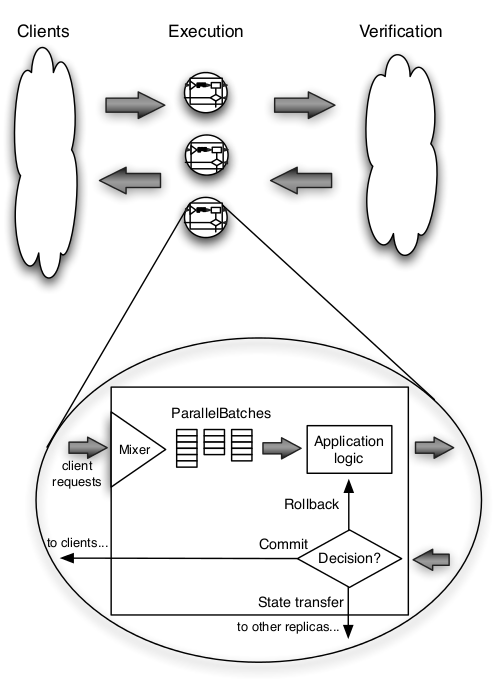
\includegraphics[width=0.75\textwidth]{eveOverview.png}
\caption{\label{eveDiagram} An overview of the Eve protocol as it appears in the original paper \protect\cite{eve}.}
\end{figure}

In theory the execute-verify approach is straightforward, but in order for Eve to work well, it is important that the case that requests have to be re-executed in a sequential manner is rare. 
If this were not the case, Eve would be strictly worse than SMR implemented sequentially because of the need to execute requests multiple times to guarantee safety. 
To reduce the likelihood that request interleavings cause the final states of replicas to diverge, the authors introduce what they call the mixer (discussed in Section \ref{EveMixer}). 
After Eve runs the mixer on the incoming requests, it proceeds to the execution stage described in Section \ref{EveExecution}. 
After executing a batch of requests, Eve moves on to the verification stage which guarantees that replicas compare their states efficiently and in a way that tolerates even Byzantine failures. 
This verification stage is described in Section \ref{EveVerification} and the final results that the authors are able to produce with Eve are presented in Section \ref{EveResults}.

\subsection{The Mixer}\label{EveMixer}
Given a set of requests submitted to each replica in the Eve system by the current primary, each replica's mixer constructs a batch of requests to schedule for execution in the following way. 
The mixer examines each request to determine if it conflicts with any request already added to the next batch to execute. 
If the request does not conflict, it adds the request to the next batch to execute. 
If it does conflict, the mixer passes over the request. 
After a complete pass, the mixer releases the batch to be executed and after doing so, repeats this process on the requests that were left out of the batch on the previous pass.

The authors found that mixers were both easy to implement for various real applications such as the TPC-W benchmarks, and greatly reduced the likelihood that replicas would diverge because of thread interleavings \cite{eve}. 
It is important to note that while the mixer does improve performance of the system greatly, it is not needed for either the safety or liveness conditions of SMR. 
Because Eve can re-execute requests sequentially as a fallback, there is no requirement that the requests in a batch do not conflict and therefore there is no required accuracy of the mixer in order for Eve to be correct.

\subsection{The Execution Stage}\label{EveExecution}

The execution stage in Eve is where the system gains its massive performance improvements over a sequential agree-execute SMR system. 
The output of running the mixer on the set of client requests is a batch of requests that are unlikely to cause replicas to diverge. 
This could possibly happen (and is much more likely without a mixer) because of non-deterministic interleavings of the operations performed by the parallel threads.
In the execution stage, these requests are distributed out across a number of execution threads to be run in parallel concurrently. 
When all of the execution threads in a replica finish performing the commands specified by the client requests in the batch, a hash of the final state of the state machine is computed efficiently using a deterministic Merkle tree implementation. 
This hash of the final state is then used in the verification stage to determine whether or not the parallel execution caused a divergence in the final states of the replicas.

\subsection{The Verification Stage}\label{EveVerification}
In Eve's verification stage, replicas must compare their final states in an efficient manner that is also resistant to even Byzantine failures. 
This is accomplished by relying on cryptographic primitives such as Message Authentication Codes (MACs) and collision resistant hashes of the states \cite{eve}. 
As mentioned in the previous subsection, Eve replicas compute a hash of their state after processing a batch of requests by each using a deterministic Merkle tree for efficiency \cite{eve}. 
After computing the root hash of the tree, replicas sign and send to a separate set of verification machines a signed token that consists of the root hash they started with before processing the current batch, and the hash of their state after processing the batch in a parallel manner.

The verification machines then run an agreement protocol on the tokens (which are the hashes of each replica's state) submitted to them by all the replicas. This protocol is explained at length in Kapritsos' doctoral thesis and the original Eve protocol paper \cite{manosThesis, eve}.
During this agreement protocol, the verifiers can decide that a view change is required which allows this system to tolerate even Byzantine failures \cite{upRight}.
At the end of agreement in the simple case, all of the tokens  match and the verifiers instruct the primary to release the result of the computation to the clients. 
This is achieved by responding to the replicas with a ``commit" message. 
If instead some tokens differ but there is a token that enough replicas submitted to guarantee that a correct replica submitted it, the verification machines respond with a commit for that token but require the replicas that did not reach that state to receive a state transfer from the replicas that did. 
This state transfer is performed in an incremental manner, allowing Eve to save considerable bandwidth for this operation.

In the worst case, the verifiers do not identify a token that was reached by enough replicas. 
In this case, the verifiers require all replicas to re-execute the requests in the batch in a sequential manner. 
When this case arises, a view change is also performed and the primary replica is rotated to ensure progress.
After the replicas have re-executed the requests in the same order, there is no need to enter the verification stage again because the execution was performed deterministically. 
This deterministic execution guarantees that all replicas arrive at the same ending state.
Note that this verification stage maintains the liveness property, since it is impossible for the replicas to get stuck in an infinite loop of verification.

\subsection{Performance Results}\label{EveResults}

The experimental evaluation of Eve shows promising results for this approach to a multi-threaded replicated state machine. 
In particular, the designers of Eve demonstrate with microbenchmarks that Eve is capable of a 12.5x speedup over sequential execution using 16 core machines with 10ms requests. 
These numbers do however fall slightly with lightweight requests. 
They find that the improvement decreased to 10x for 1ms requests and 3.3x for 0.1ms requests mainly because of the inability to saturate the system with client requests and the increased overhead of the checkpointing system relative to the time spent performing computation for each request.

The authors also compare Eve's performance to an existing attempt at performing multi-threaded SMR called Remus \cite{remus}. 
In Remus, the primary replica executes client requests with multiple threads and then transfers its entire state to the other replicas. 
This approach, referred to as passive replication, both requires considerably more bandwidth than Eve (because of the transfer of full states) and does not protect against commission failures, while Eve does. 
Eve is shown in the authors' tests to outperform Remus throughput wise by a factor of 4.7x while using orders of magnitude less network bandwidth.

\chapter{Adam: State Machine Replication with Communicating Services}\label{Adam}

Systems such as Eve can be used successfully in a parallel environment to achieve serious performance improvements in terms of request throughput however systems today are rarely well described by the simple client-server model that Eve adheres to.
Instead, most services need to interact with other services while processing a request from a client \cite{tao, spanner, dynamo}. 

For example, if a client visits a cloud file storage website \cite{dropbox}, the server handling the client's request needs to make what we will refer to as a ``nested request'' to a separate service. This nested request might function to retrieve the names of the client's files, before sending the contents of the webpage back to the client. Figure \ref{anatomy} shows the anatomy of a client request that we will be considering for the for the rest of this paper. In the diagram, the local computation can be thought of as as the time that the webserver spends rendering the HTML to return and the remote computation can be thought of as the remote service loading the user's files.

\begin{figure}[h]
\centering
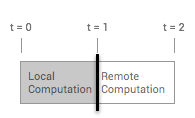
\includegraphics[width=0.5\textwidth]{RequestAnatomy.png}
\caption{\label{anatomy}The anatomy of a client request that must perform a nested request. The dark line is used to indicate a checkpoint operation. We say that a request requires two time slices to complete for simplicity: the first for the local computation and an equal amount of time for the remote computation.}
\end{figure}

Eve's approach to multi-threaded SMR successfully leverages the multicore nature of today's machines, but it is not immediately clear how to extend such a system to allow for replicated services to communicate. 
In this chapter, we will explore the previous work that was performed to convert the Eve system to work in this new environment: one where servers not only expose their states to clients, but also to other services through nested requests.

\section{System Model}
We will assume a system model similar to that of Eve. 
Adam requires periods of synchrony in an asynchronous environment to guarantee liveness. 
In these periods of synchrony we will assume that messages sent between two correct processes are delivered within a bounded time. 
Outside of these periods, Adam tolerates arbitrary network delays and lost messages without violating safety.

The Adam prototypes described in this paper can be independently configured with their own fault tolerance parameters. 
Just as the UpRight system \cite{upRight}, Adam is guaranteed to respond to clients in the presence of at most $u$ failures (commission or omission) and guarantees that any response sent to a correct client is correct in the presence of up to $r$ commission failures and any number of omission failures. 
We will assume that no failures in the system can break cryptographic primitives which could for example allow failed nodes to forge a correct node's MAC. This assumption was also made in Eve \cite{manosThesis, eve}.

\section{Initial Approaches}

Before describing Adam, it is important to understand why speculative execution SMR approaches such as Eve do not work in this environment with communicating services. 
Consider a service $A$ that is using Eve and is processing client requests. 
While processing some client requests, $A$ must make a call to a separate service $B$. 
Now suppose that because of the speculative nature of Eve, too many replicas diverge while processing this client request. In Eve, this causes all replicas to rollback to their state before they began processing the client requests and try again in a sequential manner. 
At this point, the request that service $A$ made to $B$ has already happened and cannot be rolled back. 
If service $B$ had clients of its own, they could see the result of this nested request even though service $A$ was rolled back. 
Worse still, when service $A$ re-executes the requests sequentially, there is no guarantee that it makes exactly the same nested request. 
Non-determinism caused by thread interleaving could result in a nested request made as a result of the same client request that is different from the nested request that is made when processing sequentially.

This well-known problem is known as the \textit{output commit} problem \cite{mootaz} and a very simple solution to the problem is to always take a snapshot before producing output or exposing internal state to any outside observer. 
The first attempt to convert Eve to work in this communicating services setting takes exactly this approach, and is described in Section \ref{EveModification}. 
A separate idea to achieve higher performance in this setting is to simply run in a deterministic and sequential manner, but to leverage deterministic pipelining for increased performance. 
With this idea, Adam would not be speculative and no rollback would ever be needed to maintain correctness. 
This second approach is described in Section \ref{STP}.

\subsection{Naive Sequential Implementation}

The simplest way to imagine implementing SMR in this environment would be to use the typical agree-execute approach.
This approach would work, however we will see in the next few sections that we can do much better. 
Figure \ref{NaiveSequential} shows what such an implementation would look like if it were executing $12$ client requests. 
Since an agree-execute implementation does not use speculative execution, no checkpoints are needed in this approach; however while remote computation is happening, no local computation can be performed.
As a result, the execution of $12$ client requests that incur an equal amount of work on the local and remote services (a simplification we will use for ease of explanation) takes $24$ time slices.

\begin{figure}[h]
\centering
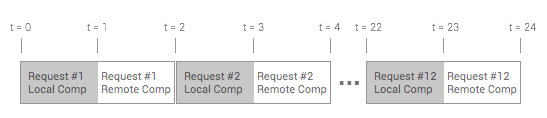
\includegraphics[width=1.0\textwidth]{NaiveSequential.png}
\caption{\label{NaiveSequential}An example execution of $12$ client requests with a naive sequential implementation. No checkpoints are needed for this approach.}
\end{figure}

\subsection{Eve Modification}\label{EveModification}

In an effort to leverage the performance gains that speculative execution approaches such as Eve promise, the first attempt to construct Adam focused on solving the output commit problem that Eve faced in this environment. 
To do this, the initial Adam contributors at the University of Texas at Austin modified the existing Eve implementation to take checkpoints before making nested requests. 

For the purposes of illustration consider an Eve-like system with multiple execution threads that are processing client requests in a speculative manner. 
When the execution threads arrive at the part of processing the client request that requires a nested request to another service, they inform the system of their progress and wait.
We will refer to a thread reaching a point where it must checkpoint as ``hitting the wall'' throughput the remainder of this paper.
After the last thread reaches such a point, the system computes a hash of its state and verifies that all replicas are consistent in exactly the same way that Eve does after processing an entire batch. 
If all replicas are in the same state after processing these prefixes of the client requests, the threads could safely make their nested requests and continue executing until the next time that they make a nested request, or until the end of their last request.

\begin{figure}[h]
\centering
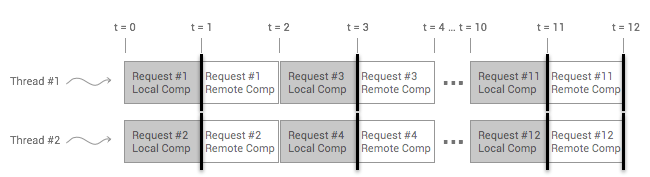
\includegraphics[width=1.0\textwidth]{Parallel.png}
\caption{\label{parallel}An example execution of $12$ client requests with the modified Eve parallel approach. For $12$ requests on two execution threads, $12$ time slices are used and seven total checkpoints (three of which are not pictured) are performed.}
\end{figure}

Figure \ref{parallel} shows what an execution of $12$ client requests would look like with this implementation using $2$ execution threads. 
Notice that checkpoints are taken right before the execution threads begin to make their nested requests to the remote service. 
Also notice that an additional checkpoint is needed at the end to make sure all replicas have the same state at the end of the batch.
This implementation (with two execution threads) finishes the batch of $12$ requests in just $12$ time slices.
Theoretically this would mean a 2x increase in performance when compared to the $24$ that the naive approach requires.

\subsection{Single-Threaded Pipelining}\label{STP}

Kapritsos et al. also designed and implemented a prototype system that leverages single-threaded deterministic pipelining to try and solve this issue. 
The advantage of pipelining is that when a single thread is processing client requests and makes a request to a separate service, it must wait synchronously for the response. 
If this communication with the remote service takes as long as the computation that the first service must perform, the system will be idle approximately half the time.
Therefore it is clear that if it is possible to perform more work while waiting for a nested request's response, the performance of the system will increase.

\begin{figure}[h]
\centering
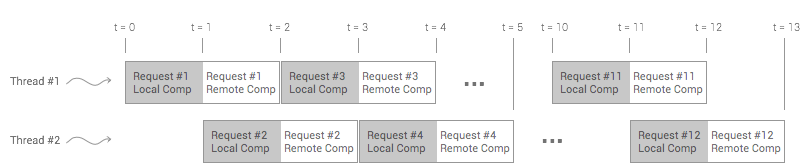
\includegraphics[width=1.0\textwidth]{SequentialPipelined.png}
\caption{\label{seqpipe}An example execution of $12$ client requests with the single-threaded pipelining approach. For $12$ requests on two execution threads, $13$ time slices are used and no checkpoints are performed because all execution is deterministic.}
\end{figure}

To build a system that performs pipelining, Kapritsos et al. use multiple threads for ease of implementation but only run them one at a time and schedule them in a deterministic way. 
Deterministic scheduling and only having a single execution thread running at any point in time guarantees that all requests are executed deterministically, and therefore that all replicas in the system converge without the need for checkpointing or potentially rolling back.

In Figure \ref{seqpipe} the execution of $12$ client requests in a single-threaded pipelined system is depicted. Notice that the grey rectangles indicate local computation, or that the replica machine is actually performing work locally. Only one thread is ever performing local computation at a time (guaranteeing determinism), but because of pipelining, the total number of time slices needed is cut almost in half over the naive approach.

\section{Initial Results}

The initial findings in terms of the performance gain that applying speculative execution or pipelining techniques had over a naive sequential implementation in this environment with communicating replicated services were quite promising. 
In Kapritsos' doctoral defense, he reported that the throughput of this speculatively executing Adam system steadily increased with the number of cores according to the microbenchmarks that he ran \cite{manosThesis}. 
Even though the throughput increased, it did not seem to be scaling particularly well with the number of cores. 
Servers with 16 cores running 16 execution threads in this implementation of Adam only had about 4 times the throughput of the same servers running with a single thread each.

The single-threaded pipelining technique described above also showed great potential. 
For very short client requests (0.1ms each), the service managed to achieve even more than the expected double throughput gain, probably because of the remote service batching requests creating what acted in practice like an additional pipeline stage. 
For requests that took longer to process (1-10ms each) however, the system successfully achieved an approximately double throughput increase because of the two stage nature of the pipeline: the first being the local computation and the second being the computation on the remote service.

\chapter{Multi-Threaded Pipelining in Adam}\label{AdamDesign}

\section{Design Overview}

The core of the work that we performed was to adapt the initial work on the Adam project to support both multi-threading and pipelining simultaneously.
As discussed in Chapter \ref{Adam}, initial work on Adam had yielded some promising results both with the multi-threaded non-pipelined approach and the single-threaded pipelined approach. 
To better understand our approach to combining these techniques, please note that a \textbf{group} of threads are execution threads that will run concurrently within the pipeline.

\begin{figure}[h]
\centering
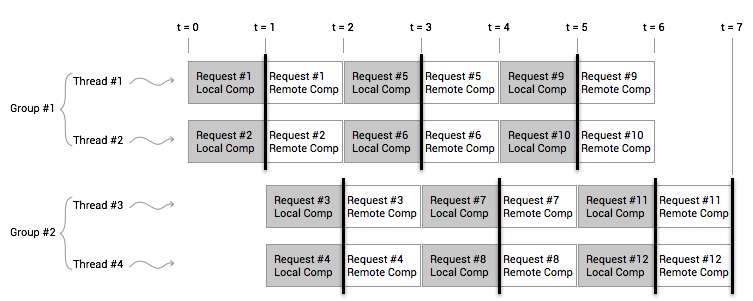
\includegraphics[width=1.0\textwidth]{PipelinedParallel.png}
\caption{\label{parpipe}An example execution of $12$ client requests in the multi-threaded pipelining approach we implemented. Two groups of two execution threads each can process $12$ client requests in just seven time slices.}
\end{figure}

At a very high level, our approach is to adapt the existing single-threaded pipelining code to have it schedule groups of threads to run in the pipeline instead of a single thread. 
To manage each group of threads, we adapt the existing multi-threaded non-pipelined Adam code to allow it to behave within this pipelined environment. 
Chapter \ref{AdamImplementation} explains at length the steps we took to convert the existing code we started with, as well as the new code we wrote to make this idea a reality.

Figure \ref{parpipe} shows what an execution of $12$ client requests looks like in our multi-threaded and pipelined system with two groups of two execution threads each. 
Notice that only one group is performing local computation at a time (the dark rectangles) but multiple threads within a group are running simultaneously.
Also notice that the full execution of all $12$ client requests requires only seven of the same time slices used in the other diagrams.
This abstraction also does not affect the total number of checkpoints that must be performed from the original multi-threaded approach.

\section{Theoretical Benefits}

By combining both pipelining and multi-threading, we expect our speedups over a naive replicated state machine in this system model to both scale linearly with the number of execution threads per group as well as double because of the two stage pipeline. 
In total this meant that with the 16 core machines we had available to test with, we hoped to see approximately 32 times the throughput of a naive sequential implementation in our microbenchmarks. 

Figure \ref{parpipe} is an example of the improvement that we would generally expect by using two groups with just two execution threads each on a batch of $12$ requests.
Notice that since only two execution threads are performing local computation at any point in time, our system only utilizes two cores on the execution replica's machine.
We would expect a 2x throughput increase from using two threads concurrently as well as approximately a 2x throughput increase from the two stage pipeline for about a 4x throughput increase over the naive sequential approach.

Visually, this is exemplified by the number of time slices in each diagram of this paper.
The naive sequential implementation (Figure \ref{NaiveSequential}) required $24$ time slices while the execution in our system required only seven.

\begin{align*}
24 / 7 \approx 3.43
\end{align*}

This number actually converges to the desired 4x as the number of requests run in each batch increases to infinity.
A formal proof of this fact is available in Jim Given's thesis \cite{jim} but conceptually it can be seen that the larger the number of requests that each thread must execute, the less the ``unmatched'' slices at the beginning and the end of the batch contribute. 

\chapter{Adam Implementation}\label{AdamImplementation}

\section{Initial Code Structure}\label{existing}

When we began our contributions to the Adam project, prototype implementations existed for both approaches described in Chapter \ref{Adam}. 
Before explaining our work to create a multi-threaded pipelined SMR system that uses speculative execution, we examine in detail the existing building blocks that we use to construct our final implementation.

\subsection{Existing Multi-Threaded Adam Implementation}\label{BM}

The existing multi-threaded Adam implementation we started with was a modification to the existing Eve \cite{eve} code that allowed the code to perform nested requests. 
Some of the core changes involved the use of Apache's Commons Javaflow library \cite{javaflow} to easily allow execution threads to rollback their state to a checkpoint, even if they were currently performing a local execution. 
The other modifications to Eve involved adding support for multiple checkpoints taken per batch, one after every time the execution threads ``hit a wall'', meaning that all currently active execution threads were either finished with the entire batch of requests or were ready to make a nested request.

Execution threads were controlled in this implementation by the Batch Manager (BM) which handled the logic of making sure all threads had ``hit a wall'' and initiated the checkpoint operation for each execution thread. 
This BM was also intended to handle ensuring that the all replicas were at the same state at each wall, which involved sending off a hash of the replica's state and initiating a rollback if needed. 
When we received the code however, this verification process was largely not finished as the existing multi-threaded attempt was intended to simply demonstrate that speculative execution could still provide performance gains even with communicating replicated services.

\subsection{Sequential Pipeline Manager}\label{SPM}

The Sequential Pipeline Manager (SPM) was first implemented by Kapritsos to demonstrate that the single-threaded pipelining approach had promise in this system model. 
The SPM in particular was the part of the system that controlled which execution thread was currently running and handled scheduling the next thread when the active thread desired to yield.
This meant that the SPM was also responsible for enforcing the condition that only one execution was being performed at any point in time and that all execution was deterministic.
This code was very straightforward but it served as the inspiration for the more complex pipeline manager that we built later to schedule groups of threads.

The SPM began the execution of a batch of requests by deterministically assigning requests to each thread in a round-robin fashion.
Even though the pipeline executed sequentially, the SPM used many lightweight threads to simplify the scheduling process. 
After assigning work to threads, the SPM notified the first thread to begin. 
That thread would then start processing the client request until it was ready to make a nested request. 
The active thread at this point would then call a yield function in the SPM to notify it to schedule the next thread. After notifiying, the active thread would immediately make a blocking call to the remote service. 
When the SPM received this yield notification, it notified the thread with the next higher id (modulo the number of threads) to begin execution. 
Eventually, the last thread with work to do would yield the pipeline, at which point the SPM would schedule the first thread again. 

The first thread would then either continue waiting for the nested request to complete, or would continue executing the client request to completion. 
After completing a client request, the active thread would either start executing its next assigned request or would notify the SPM if it had executed all of its assigned requests.
Once all threads had responded in this way, the SPM would finish the batch and release the results to the clients after which it would begin the next batch.

\section{Core Components}

To implement Adam with the multi-threaded pipelined approach, we first combine the two existing approaches into one system before implementing the parts of the functionality that were not yet present. 
We begin by adapting the Sequential Pipeline Manager (SPM) to schedule groups of threads instead of just individual threads, and then modify the Batch Manager (BM) to control a group of execution threads that can be scheduled onto and off of the pipeline.
After these modifications, we finished implementing parts of Adam that had not been implemented for the initial proof of concepts such as the verification stage and made appropriate modifications to other existing parts of the code base to support both multi-threading and pipelining simultaneously.

\subsection{The Parallel Pipeline Manager}

By taking the structure of the existing SPM written by Kapritsos (and described in Section \ref{SPM}), we build what we call the Parallel Pipeline Manager (PPM) to schedule groups of threads in the context of the pipeline. 
The changes that we make to the SPM to control groups of threads mostly center around initialization and the detection of the correct time to swap groups on to or off of the execution pipeline.

Within the SPM, a simple mechanism was used to schedule client requests to execution threads that ran one at a time in a pipelined fashion. 
Essentially, the SPM would assign the requests to threads by giving each thread one request before giving the first thread a second request and so on. 
In the PPM, we instead must schedule requests within a batch to both groups of threads and to threads within those groups. 
This is performed after the mixer has been run on the batch, so we are able to assume that requests are mostly non-conflicting. 
We experimented with a couple of ways of assigning the requests to the threads but eventually found that our system works best when we assign every thread in the first group a request before beginning to assign requests to threads in the second group.
We continue this process with the remaining groups before assigning a second request to each thread within the first group. 
We believe that this is the best way to assign the requests because assigning them in this way makes sure that all cores are utilized as best as possible, leveraging the multicore nature of the machine before taking advantage of the pipelining by using multiple groups. This claim is argued more formally in Jim Given's thesis \cite{jim}.

The SPM also had a method that execution threads could call when the active execution thread was about to make its nested request and was ready to yield the pipeline to the next thread. 
In the PPM, this procedure is slightly more complicated because the PPM must wait for all threads to be in a state that they can yield the pipeline in. 
Each execution thread makes the same sort of yield request, but the result of the function call is simply a flipped bit in a bitarray that stores which threads are ready to yield. 
When the last thread in the currently active group (the group that the PPM is allowing to execute) calls this yield function, the last thread notifies the PPM's control thread.
This control thread then realizes that it is time to schedule a new group of threads to run and updates the active group accordingly. 

This bitarray also must be updated when threads no longer want to yield and are ready to execute again (e.g. when the nested request returns for a thread). 
We decide in our implementation to only allow the PPM's control thread to mark when threads no longer want to yield because of the following scenario. 

Imagine that in a group of two execution threads, the first thread reaches the point where it is ready to yield and makes its nested request.
Pretend that the second thread requires more local computation time and therefore is slightly behind the first thread in making its nested request.
The second thread then does not reach the point to yield before the nested request that the first thread made returns.
If we allow the first thread to mark that it no longer wants to yield the pipeline (since its nested request had completed), the PPM will not schedule the next group of threads to execute because not all of the threads in the currently active group want to yield anymore.
This is an issue because the second request's remote computation could take a long time, in which case no thread is currently executing on the local machine and the entire local service is therefore idle.
A simple workaround for this is to only allow the PPM to mark the active group's threads as not wanting to yield after they have been swapped off the pipeline at least one time.

\subsection{The Parallel Group Manager and Execution Thread Modifications}

The second part of our system that enables groups of threads to run in a speculative manner is the Parallel Group Manager (PGM). This part of the system controls the execution threads within a single group.
It is at this layer of abstraction in our system that we handle taking checkpoints, possibly rolling back, and informing the PPM when all of the threads in the group are finished executing their assigned requests within the batch.
The Batch Manager (described in Section \ref{BM}) served as our starting point for this part of our implementation, as it was already designed to control multiple execution threads in the Adam environment.
Some of the major modifications we make to the existing BM code involve making sure that the PGM was able to be scheduled onto and off of the pipeline controlled by the PPM, and that verification was performed in a way to guarantee safety and liveness. 
Providing these correctness guarantees involves making sure that verification requests are made at all of the required times and that the responses to these messages are handled properly. 
More details about our verification modifications and how we handle rollback in this approach are described in Section \ref{Verification}. 

In order to make sure that PGM does not continue executing after being swapped off of the pipeline, we require that it communicate with the PPM to determine the number of the currently active group. 
If the active group number corresponds to the group controlled by the PGM and its corresponding control thread, the PGM continues instructing the execution threads to process more requests and to take checkpoints when needed. 
If instead the PGM finds that the current group is no longer its own, it simply waits until the PPM notifies it to continue.

We also make many changes to the execution threads to ensure that they behave in this both parallel and pipelined system.
For example, we ensure that the execution threads make the appropriate calls into the PPM to notify the PPM when they are ready to yield and that the threads ensure that it is their corresponding group's turn to execute in the pipeline before proceeding with their own executions.

\subsection{Verification Stage}\label{Verification}

When we inherited the existing proof of concept Adam implementation, the verification stage had yet to be converted from its original behavior within Eve.
In Eve, the system was only required to send out a verification message at the end of the computation of a batch to ensure that all replicas converged \cite{eve}.
In Adam however, the verification process must be performed before any execution thread makes a nested request as well as at the end of the batch because both of these situations expose intermediate state to potential clients.

% There was a sentence here about adding extra threads being a bad thing: This was the case with threads that were spinning inefficiently
% but after we eliminated these troublesome issues, this was no longer the case

In order to make this modification, we first add a second message processing thread to the system that can concurrently process the responses from a verification stage, while another thread is processing incoming client requests.
When the verification responses are received from the verifiers by the execution replicas, they process each response and determine whether they need to rollback, receive a state transfer, or could safely continue executing in the same way. 
This part of the verification stage works almost like Eve's which is described in Section \ref{EveVerification}.
\section{Rollback and Correctness Guarantees}

In this parallel pipeline system we must be prepared to rollback the state of an Adam replica to arrive at one that all replicas agree on in the event that the speculative execution causes a divergence. 
Note that because we always ensure that all replicas are in the same state immediately before making any nested request, this means that the state that we must rollback to in the case of divergence is either right before some execution threads make a nested request or right at the beginning of a batch. 
If it is the latter, rollback is trivial, we simply throw away all work performed so far and execute the requests again in a sequential deterministic manner to guarantee that progress is made and that all replicas converge. 
This deterministic execution can even be performed in a sequential pipelined manner to achieve better performance than a naive sequential approach.

If instead we rollback to right before the threads in a group make a nested request, our system restores the state of all execution threads to the state they had when the latest checkpoint was taken. After doing so and setting the new active group successfully, the system switches all threads into a sequential deterministic mode to ensure progress and convergence.
We use Apache's Commons Javaflow library \cite{javaflow}, specifically the Continuations objects in this library, to checkpoint the stack of each execution thread.
In addition to the stack, Adam also requires that the objects referenced in the stack are deep copied to the Merkle tree, an operation that is automatically performed simply by annotating the prototype code.
This allows us to restore this stack and all referenced objects during a rollback and guarantee that all execution threads are in the exact state they were in right before the nested request was made on each replica.
These Continuation objects with the stack of each thread are stored in the same deterministic Merkle tree data structure that Eve used which allows the replicas to make sure that they also have the same recorded stacks for each execution thread whenever a verification is performed.
This also allows replicas to receive continuations in a state transfer and immediately start the execution threads at the same point in the execution. 

After performing a rollback in the non-trivial case, the threads in the now current group re-execute their nested request with the same sequence number that they used the first time which allows the remote service to respond from a cache and not perform operations multiple times.
Since we know that all execution threads were in the same state before making this request, we know that the request that each execution thread makes is exactly the same, thereby eliminating the issue that Eve has in this environment with making requests that might never be repeated after rolling back \cite{manosThesis}.

\chapter{Evaluation and Results}\label{AdamResults}

When we finished implementing the multi-threaded and pipelined version of Adam, we were dismayed to find that our throughput increase results were much lower than we had hoped. 
For a variety of reasons, we first saw that using eight threads in Adam only resulted in less than a 4x throughput increase over the naive sequential implementation for very large requests when we expected something closer to a 16x improvement. 
We then took a methodical journey through several heinous bugs and the intricacies of this design until we arrived at much more satisfying performance results. 
For details on the approach we took to correcting our implementation, and more about the problem that we are trying to solve in general, please read Jim Given's thesis \cite{jim}.

We perform the evaluation we present here on a testbed of several Dell PowerEdge R200 4 x 2.4GHz Intel Xeon machines and three Dell PowerEdge R515 16 x 3.2GHz AMD Opteron machines. 
We use the 16 core (R515) machines as our execution replicas and the four core (R200) machines as our verifier, client, and filter machines. 
Because we only have three 16 core machines, we are only able to perform scaling studies up to 16 cores in an unreplicated setting (meaning we tolerate no faulty execution replicas) with one 16 core machine running as the local service and another as the remote service. 
For these unreplicated studies, only the execution nodes are not replicated, all verifier machines are still replicated in a fault tolerant way (four total to handle one commission error). 
We performed the fully replicated study we describe in this chapter by using each 16 core machine as both a 8 core local replica and an 8 core remote replica which constrains us to only being able to test in a full setting (with $r = 1$) with up to 8 execution threads.

\begin{figure}[h]
\centering
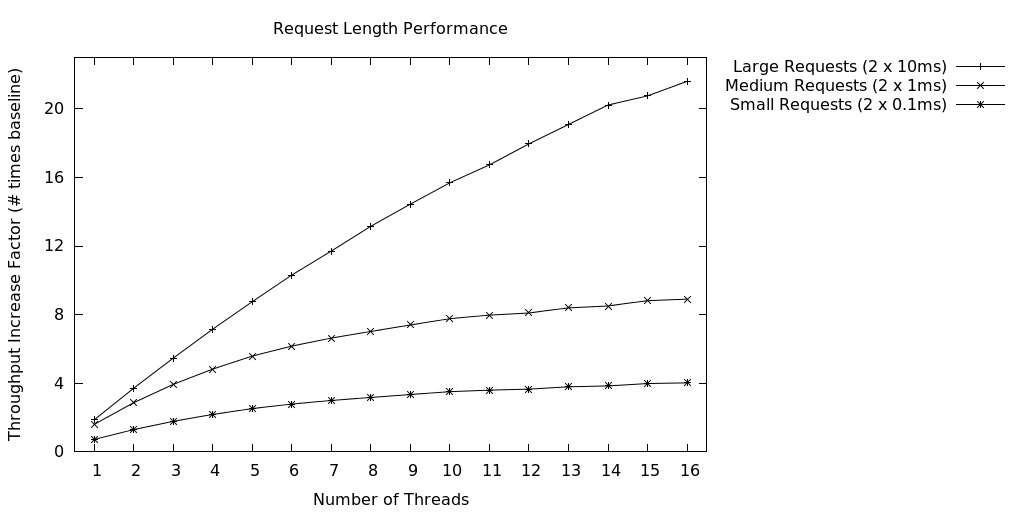
\includegraphics[width=1.0\textwidth]{graphs/requestweights/graph.png}
\caption{\label{scaling}Adam speedup over sequential performance for small, medium, and large requests.}
\end{figure}

One of our chief concerns when we evaluate the performance of our system is to see how the system scales with additional parallel execution threads. Figure \ref{scaling} shows the factor of throughput increase that we achieve by adding more execution threads to our system in an unreplicated environment.
These numbers are obtained by running our system with three groups of $x$ threads each where $x$ is the number found on the horizontal axis. 
We then take the saturated throughput of the system for each number of threads and divide it by the throughput that a naive sequential implementation achieves for each size of request.
As mentioned in Chapter \ref{AdamDesign}, we expect the theoretical maximum benefit of our system to be 32 times the throughput of the baseline, gaining a factor of 16 improvement from utilizing 16 cores and then doubling the throughput because of the two stage pipeline.
We come closest to this theoretical maximum with large (10 ms local computation and 10ms remote computation) requests which is because the increased computation time helps mask the overhead introduced by the checkpointing and the verification stage.
We deviate from the theoretical benefit even more for shorter requests as the overhead becomes more pronounced and possibly because of bottlenecks in the system when processing larger numbers of client requests that we have not yet identified.

\begin{figure}[h]
\centering
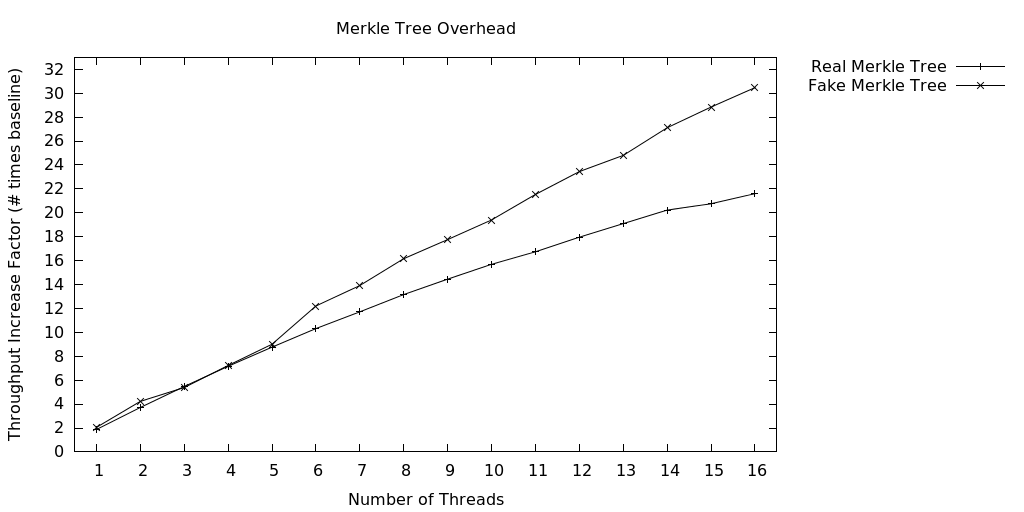
\includegraphics[width=1.0\textwidth]{graphs/merkleimpact/graph.png}
\caption{\label{scalingmedmerkletree}Merkle tree impact on throughput relative to the sequential execution baseline for large requests.}
\end{figure}

As Figure \ref{scalingmedmerkletree} shows, the Merkle tree implementation that we use appears to be a major source of overhead in this system.
In this graph, we compare the scaling behavior of the unreplicated system when using a real Merkle tree implementation to when we use a fake Merkle tree.
With the fake Merkle tree, we perform all of the identical operations that we perform with the real tree but all hashing and Merkle tree versioning operations complete instantly.
With the fake tree in this unreplicated setting we achieve a maximum of just over $30$ times the throughput ($1371$ requests per second) of the naive sequential baseline execution ($45$ requests per second) out of a theoretically possible $32$ times the throughput.
For the real tree, we achieve a speedup of almost $22$ times the baseline ($972$ requests per second) with all $16$ cores, meaning that we are losing nearly $400$ requests per second because of the overhead of the Merkle tree's operations.
As a result, we believe that there is still room for improvement through optimizations of our Merkle tree implementation.
This could be achieved through better detection of new objects in the replica that must be hashed or more intelligent space allocation within the tree itself.

\begin{figure}[h]
\centering
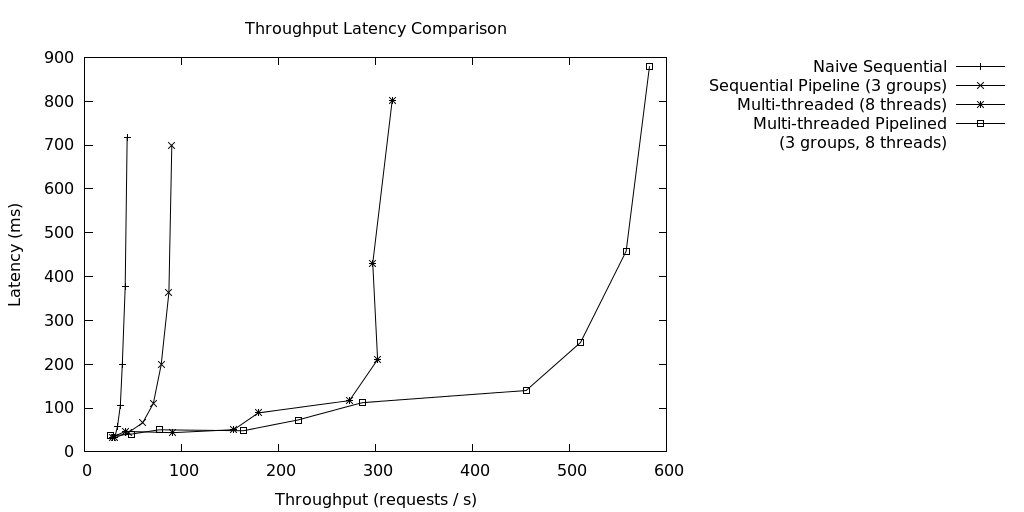
\includegraphics[width=1.0\textwidth]{graphs/latencythroughput/graph.png}
\caption{\label{head2head}Latency-Throughput graphs of Adam for large requests with all four approaches.}
\end{figure}

We also compare our Adam implementation head to head with the previous three approaches described in Chapter \ref{Adam}: the naive sequential approach, the single-threaded pipelined approach, and the multi-threaded non-pipelined approach. 
Figure \ref{head2head} shows latency throughput graphs for our implementation running with three groups of eight threads each in a fully replicated environment. 
We compare our implementation in this graph to the multi-threaded but non-pipelined approach running with eight threads, with the single-threaded pipelined approach running with three threads (which is equivalent to our implementation using three groups), and with the naive sequential implementation. 

It can be seen from the graph that the naive sequential implementation achieves close to $50$ requests per second which is the theoretical maximum throughput for $20$ms requests ($10$ms for the local and $10$ms remote computation). 
The sequential pipelined approach approaches twice the performance of the naive implementation because of the fact that the pipeline is of depth two (the local service and the remote service).
The original multi-threaded Adam approach achieved a throughput of just over $300$ requests per second with eight execution threads. We would expect in this scenario at most an 8x increase in throughput over the naive sequential approach which would mean a throughput of $360$ requests per second.
We miss this mark by a little more than one multiple of the naive sequential approach throughput because of to the added overhead of the verification stage.
Our multi-threaded and pipelined implementation achieves a maximum throughput of at most $582$ requests per second with this setup while the original multi-threaded approach achieves slightly over $300$ at its saturation point. 
This shows that our pipelining improvements achieve close to the throughput doubling that we expect.

\chapter{Future Work}\label{FutureWork}

One proposed improvement to the described design that we did not implement is an optimization for the verification process.
The idea is to combine the nested requests with the verification requests, eliminating the need for the verifiers and the extra round trip they require.
This approach does however require that the remote service is aware that the service making nested requests might have failures of commission while currently the remote service just has to treat Adam as a client that might make repeated requests with the same sequence numbers. 
In practice, we found that this round trip was not the bottleneck of the system, but this improvement could still easily be made.

As shown in our evaluation of Adam, we did find that our system had much better performance gains on longer client requests than shorter ones because of the overhead that the additional checkpoints incurs in the form of additional Merkle tree computations. 
We believe that the system could be modified to minimize the total number of checkpoints needed by making much larger groups and not checkpointing until all of the requests in these larger groups are ready to make the nested request.

Another concern with our current implementation is the need to have large batch sizes. With three groups running in the system with 16 threads each, at least 48 concurrent and non-conflicting requests are needed to assign each thread a single client request to perform. 
To achieve the performance benefits from pipelining that we described in this paper, each execution thread must have multiple requests to process which drastically increases the needed batch size. 
One proposed solution would be to design the system so that the pipeline is always active, thereby eliminating the need to restart the pipeline with new batches and instead just adding the work to the execution threads' queues. 
We believe this is possible since we are already taking checkpoints for each request, though it complicates the rollback and work assigning procedures that we describe here.

\chapter{Related Work}\label{RelatedWork}

% Work related to Eve
This work built off of existing work from the University of Texas at Austin Laboratory of Advanced Systems Research from both the Eve project and initial proof of concept approaches to Adam. Aside from this already described related work, there has been some work in the field of replicated remote procedure calls (RPC) and work on passive replication systems.

\section{Replicated Remote Procedure Calls}

The concept of a replicated RPC has been around for decades \cite{rrpc, ftrpc}.
Such a system allows multiple replicated modules to interact through a procedure call interface presented to the system designer.
Replicated RPC was explored before advancements were made in the area of speculative execution and as a result the systems in literature rely on sequential execution (or at minimum serialization of requests) to maintain consistency between replicas. 

\section{Passive Replication}

Passive replication is a technique employed by systems such as Remus \cite{remus} that enables multi-threaded SMR. 
These techniques work by allowing the primary to perform all execution speculatively (which can be multi-threaded and therefore non-deterministic) and then have the other replicas passively absorb this state from the primary.
One downside of this approach is that it does not handle errors of commission  while systems such as Adam and Eve do.

In addition, Remus relies on aggressive checkpoint pipelining for performance that would not work in an environment with inter-service communication.
Remus performs speculative execution past checkpoint times, which allows it to buffer client outputs until the state of the primary becomes visible. 
Outputs of the system originally occurr only when the primary releases the responses to client request however in this new setting, Remus  also has to block until a checkpoint is performed to make a nested request. 
This additional blocking leaves the system idle until the checkpoint has been performed and is received by other replicas.
It is possible for Remus to be adapted to perform similar pipeline techniques to Adam but it would still suffer from its more expensive checkpointing operations and higher network bandwidth usage than Eve \cite{eve}. 

Adam uses Eve's same system for collecting state that includes only the subset of the state that determines the the operation of the state machine and ignores values that vary over the replicas such as the state of communication devices or other unimportant configuration parameters \cite{manosThesis}.
As a result, Adam has to transmit less over the network in the case of a state transfer than a modified version of Remus.
In the common case, Adam only has to transmit hashes to guarantee consistency compared to the entire state that Remus must transmit before any nested request.

\chapter{Conclusion}\label{Conclusion}

Traditional approaches to state machine replication use deterministic single-threaded execution to guarantee that replicas agree on the same final state. Although these approaches are straightforward, they fail to take advantage of the multicore nature of today's machines. 
In addition, these approaches are ill-suited to an environment with communicating services. This is because communication with other services requires a sequential execution thread to block while waiting for a response. 

Newer techniques such as the Eve protocol \cite{eve} leverage speculative execution to allow SMR systems to be multi-threaded.
Even systems like Eve however do not immediately perform well in an environment with communicating services and known pipelining techniques can be effectively used to improve performance.
We present a novel approach to providing the replicated state machine abstraction in an environment with communicating services that leverages both the multicore nature of today's machines and pipelining techniques to improve resource utilization. 

We find through the use of microbenchmarks that our design and implementation allows a workload of heavy requests to scale over $21$ times the throughput of a naive sequential implementation in a non-replicated setting with 16 core machines.
In a fully replicated and fault tolerant setting, we achieve $12.9$x the throughput of a naive sequential approach with just eight cores per execution server in our microbenchmarks.
Although our current results on smaller request sizes do not scale as well with the number of cores in the system, we believe that the issues with our system are implementation specific and are exacerbated by our lack of access to a cluster large enough to saturate our system with client requests.
We demonstrate that speculative execution based multithreading techniques can be used with communicating replicated services to scale the system with the number of cores of the execution replicas and that pipelining can be applied to these multi-threaded techniques to nearly double the performance of such a SMR system.

\bibliographystyle{plain}
\bibliography{bib}

\end{document}
